\documentclass[onecolumn, draftclsnofoot,10pt, compsoc]{IEEEtran}
\usepackage{graphicx}
\usepackage{url}
\usepackage{pdfpages}
\usepackage{setspace}
\usepackage{caption}
\usepackage{hyperref}
\usepackage[numbib,nottoc]{tocbibind}
\usepackage{geometry}
\geometry{textheight=9.5in, textwidth=7in}
\def\code#1{\texttt{#1}}
% 1. Fill in these details
\def \CapstoneTeamName{Code Monkeys in Space}
\def \CapstoneTeamNumber{		33}
\def \GroupMemberOne{			Mark Bereza}
\def \GroupMemberTwo{			Joseph Struth}
\def \GroupMemberThree{			Kevin Turkington}
\def \CapstoneProjectName{		NASA University Student Launch Initiative}
\def \CapstoneSponsorCompany{	Mechanical Engineering, Oregon State University NASA}
\def \CapstoneSponsorPerson{		Dr. Nancy Squires}

% 2. Uncomment the appropriate line below so that the document type works
\def \DocType{	%	Technology Review and Implementation Plan
				%Requirements Document
				%Technology Review
				Design Document
				%Progress Report
				}
			
\newcommand{\NameSigPair}[1]{\par
\makebox[2.75in][r]{#1} \hfil 	\makebox[3.25in]{\makebox[2.25in]{\hrulefill} \hfill		\makebox[.75in]{\hrulefill}}
\par\vspace{-12pt} \textit{\tiny\noindent
\makebox[2.75in]{} \hfil		\makebox[3.25in]{\makebox[2.25in][r]{Signature} \hfill	\makebox[.75in][r]{Date}}}}
% 3. If the document is not to be signed, uncomment the RENEWcommand below
\renewcommand{\NameSigPair}[1]{#1}

%%%%%%%%%%%%%%%%%%%%%%%%%%%%%%%%%%%%%%%
\begin{document}
\begin{titlepage}
    \pagenumbering{gobble}
    \begin{singlespace}
    	%%\includegraphics[height=4cm]{coe_v_spot1}
        \hfill 
        % 4. If you have a logo, use this includegraphics command to put it on the coversheet.
        %\includegraphics[height=4cm]{CompanyLogo}   
        \par\vspace{.2in}
        \centering
        \scshape{
            \huge CS Capstone \DocType \par
            {\large\today}\par
            \vspace{.5in}
            \textbf{\Huge\CapstoneProjectName}\par
            \vfill
            {\large Prepared for}\par
            \Huge \CapstoneSponsorCompany\par
            \vspace{5pt}
            {\Large\NameSigPair{\CapstoneSponsorPerson}\par}
            {\large Prepared by }\par
            Group\CapstoneTeamNumber\par
            % 5. comment out the line below this one if you do not wish to name your team
            \CapstoneTeamName\par 
            \vspace{5pt}
            {\Large
                \NameSigPair{\GroupMemberOne}\par
                \NameSigPair{\GroupMemberTwo}\par
                \NameSigPair{\GroupMemberThree}\par
            }
            \vspace{20pt}
        }
        \begin{abstract}
        % 6. Fill in your abstract    
        	In order to achieve the ultimate goal of scoring well in the competition, the responsibility of Code Monkeys in Space is to implement software that will allow the payload, a rover, to move autonomously and avoid obstacles, a website that will host deliverables and team information, and software for a data logger unit used in test flights of the launch vehicle that will display collected data in a human-readable way. This document will detail the high level design of these software products in terms of block-level interfaces, data organization, algorithms employed, technical definitions, and more.
        \end{abstract}     
    \end{singlespace}
\end{titlepage}
\newpage
\pagenumbering{arabic}
\tableofcontents
\listoffigures
% 7. uncomment this (if applicable). Consider adding a page break.
%\listoffigures
%\listoftables
\clearpage

% 8. now you write!
\section{Introduction}
\subsection{Purpose}
The main goal of NASA's University Student Launch Initiative (USLI) competition is to launch a rocket exactly one mile into the atmosphere with an experiment onboard as its payload. This experiment can be one of the following: "target destination", autonomous "deployable rover", or "landing coordinates via triangulation" \cite{USLI_handbook}. The OSU USLI team's experiment of choice is the deployable rover. The rover experiment only has two minimum requirements set by NASA: First, upon landing and locating the rocket the team will remotely trigger a deployment of the rover. Once deployed, the rover must autonomously (without any human assistance) move from its deployment zone to its destination at least five feet away from any part of the launch vehicle. Upon reaching its destination or before battery depletion, the rover will then deploy solar panels. As a side goal of the USLI competition, teams must conduct educational outreach with schools or clubs. Such activities may be categorized as either direct, meaning one-on-one learning exercises or activities, or indirect, meaning a single activity or exercise performed for the benefit of a group of students simultaneously. Each member of the USLI team will participate in at least one outing of educational outreach (as defined by NASA in the USLI handbook) at a local or non-local school (K - 12).
\subsection{Scope}
Overall, the goals of this competition are the following:
\begin{enumerate}
\item Construct and launch a rocket carrying a payload at least a mile (5,280 feet) above ground.
\item Have the rocket deploy a parachute and safely land within 2,500 feet of the launch point.
\item After landing and after a button press, deploy a rover.
\item Have the rover drive autonomously at least 5 feet away from the rocket landing site.
\item Have the rover deploy solar cells after being at least 5 feet from the landing site.
\item The solar cells will increase in surface area after deployment (unfold).
\item Create formal technical reports regarding rocket/payload design and present them to a NASA review panel
during several formal design review meetings.
\item Participate in educational outreach and get at least 200 individuals involved in the project.
\item Maintain a website detailing project information and hosting all competition deliverables.
The subset of these overall goals that pertain to the CS capstone students involves the research, design, implementation.
\end{enumerate}
In particular, the CS seniors on the OSU USLI team, otherwise known as Code Monkeys in Space, are responsible for goals 7, 8, and 9 and the software needed to facilitate goals 4 and 5. Furthermore, Code Monkeys in Space are responsible for the design and implementation of software that will run on a data logging module inside every test launch vehicle for the purposes of data collection, which indirectly assist with goals 1 and 2. Thus, the scope of this project for Code Monkeys in Space is limited to these facets of the competition. The others will be handled by the mechanical and electrical engineering seniors on the team.
\subsection{Summary}
Code Monkeys in Space plan to achieve the aforementioned goals by:
\begin{enumerate}
\item Creating ROS modules that will allow the rover to move autonomously, avoid obstacles and path-find based on sonar sensor and IMU readings, and determine when it is at least five feet from the rocket frame in order to deploy the solar panel cells
\item Writing Python code that will run on the BeagleBone Black data logger onboard test launch vehicles that will store sensor data recorded by multiple flight sensors including temperature, pressure, and acceleration.
\item Writing further code that will perform numerical transformations on the data logger's raw data in order to obtain useful information like time of chute deployment, G forces experienced at various stages of flight, velocity and acceleration throughout the flight, and more
\item Representing the transformed and polished data on the team website in a graphical, human-readable fashion
\item Creating, updating, and maintaining a team website hosting team information and project deliverables
\item Participating in at least four separate educational outreach activities during two months between now and the competition's conclusion
\item Aiding in the writing of technical documents and presentations required at various stages of the competition, in particular the parts pertaining to software
\item Attending team meetings and NASA review sessions
\end{enumerate}
\bibliography{bibliography}
%end bibliography
\section{Glossary}

\begin{itemize}
	\item USLI: University Student Launch Initiative, the NASA competition guiding this project.
    \item ROS: Robot Operating System, a middle-ware/software framework that assists in the creation of robotics modules by providing hardware and interface abstraction and simulation capabilities.
    \item SLAM: Simultaneous Localization and Mapping. A strategy utilized by some vehicles that simultaneously calculates the vehicle's current position and generates a map of its surroundings.
    \item I2C: Serial, packet-switched communication protocol for low-speed devices such as microcontrollers.
    \item USART: Universal Synchronous/Asynchronous Receiver/Transmitter. Chip that allows for serial communication both synchronously and asynchronously.
\end{itemize}

\section{Stakeholders and Design Concerns}
\subsection{OSU USLI Team}
The OSU USLI Team is comprised of multiple capstone teams composed of both mechanical and electrical engineering students working together to design, build, and test the launch vehicle and rover. All the team members are equally invested in the success of the project and desire to preform well in the competition. The other USLI team members are stakeholders as they will rely on the CS team to ensure the software components of the project function as needed. Just as the CS team will depend on the engineers to build the physical launch vehicle and rover, they will depend on us to write software that will run correctly and make the mission successful.
\subsection{John Lyndall}
John Lyndall is an advisor to the USLI team, and a member of the Oregon Rocketry Association which aims to educate the public and promote amateur interest in and study of rocketry. He is an outspoken advocate of educational outreach, and has supported our project by providing model rockets and supplies to K-12 students. He is a stakeholder due to his investment in the project, support of rocketry, and previous experience working at NASA. 
\subsection{Dr. Nancy Squires}
Dr. Squires is the project stakeholder and one of the main proponents of rocketry at Oregon State University. She hopes to continue to expand OSU's involvement in rocketry and the USLI competition. Even  though it is our team's first year competing, she has set high expectations for our team and wants us to win despite us being a rookie team. She hopes to build on our team's work and knowledge in future years to continue OSU's involvement in the competition and perhaps improve our performance in it.

\section{Rover}
\begin{figure}[h]
	\begin{center}
		\caption{State diagram for the rover's second movement algorithm. }
		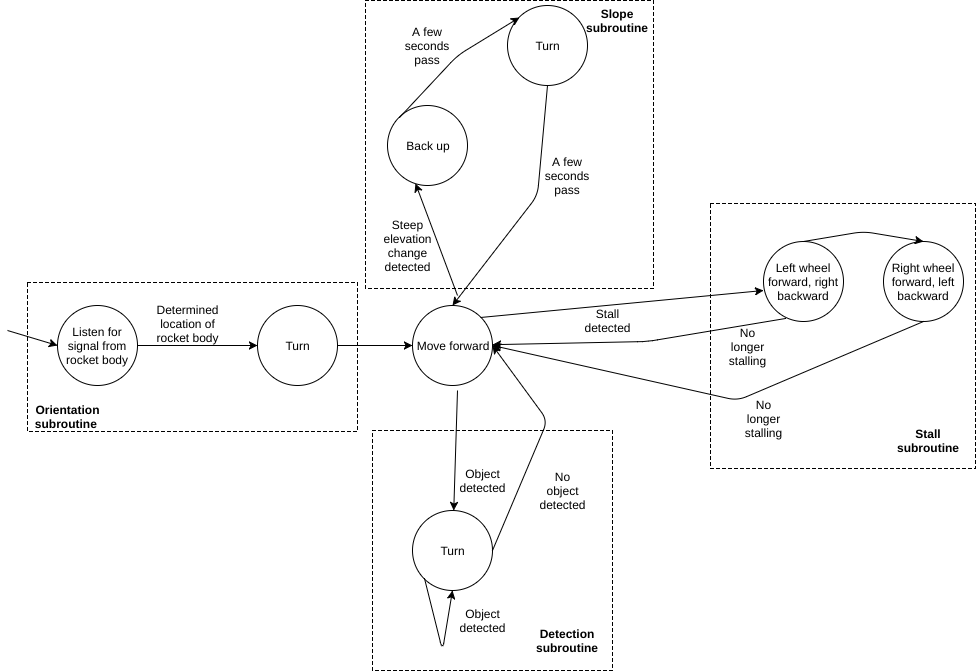
\includegraphics[width=\textwidth]{RoverStateDiagram}
	\end{center}
\end{figure}
\subsection{Design View}
The software of the rover on the bottom level will be run on the Raspbian operating system (a Debian derivative), which will serve as a resource interfacing the rover software and ROS with the Raspberry Pi's hardware components. ROS (Robotics Operating System) will be used as the link between high level algorithmic computation and I/O components, such as sonar sensors, microphones, GPS, and the IMU. ROS modules responsible for movement and path finding will subscribe to streams for these various sensors. Other ROS modules will be responsible for publishing sensor data as it arrives based on hardware interrupts to these streams. In the event of race conditions, data coming from more "vital" sensors, such as the motor driver or the IMU will take priority. 

Overall, the rover software will utilize three movement algorithms of varying complexity, The hardware needed by the less complex algorithms will be a strict subset of the hardware needed by their more complex counterparts, meaning that the rover can still function to some degree even if most of its sensors fail at a hardware level. Such redundancy is crucial when considering a rover than must function autonomously after experience extreme G forces during flight. 

The three movement algorithms are as follows:
\begin{enumerate}
\item SLAM: The rover will utilize a combination of GPS, its magnetometer, and its position relative to rocket frame parts (calculated by determining the phase shift because the same signals as recorded by the rover's two separate microphones) to triangulate its position. It will then utilize its front-facing sonar sensors combined with incremental scanning (via turning) to perform mapping of its surrounding area. Combined, this information will be used to determine an obstacle-free path for the rover away from the rocket frame that it will follow until it is at least five feet away. 
\item Obstacle avoidance: The rover will determine the location of any nearby rocket frame parts by listening for their signal on its dual microphones and then face away from them. From there, the rover will move forward, avoiding obstacles detected by its sonar sensors by turning away from them. For steep declines, which front-facing sonar sensors will not detect, the IMU will alert the rover of said decline and the rover will back up, turn away from the decline, and continue moving. At regular intervals, the rover will check it absolute direction against its initial one using its magnetometer in order to ensure that turning done during obstacle avoidance has not resulted in the rover now facing the landing site which it intends to leave.
\item Basic movement: As before, the rover will face away from the rocket if the microphones are functioning. From there, it will simply move forward continuously, only changing directions if it gets stuck, at which point it will alternate turning left and right at full power in an attempt to wiggle itself out of whatever trapped it. This strategy, corresponding to the stall subroutine in Figure 1, is also employed by the other two algorithms in the event of motor stall, but the ultimate goal of the more complex algorithms is to avoid getting stuck in the first place.
\end{enumerate}
Figure 1 shows a state diagram of the second movement algorithm listed above. The overall diagram is split into four distinct subroutines. The first, the orientation subroutine, is run as soon as the rover is ejected from its housing. It involves listening for the rocket's signal on its twin microphones and then turning until the phase shift of the signals corresponds to facing away from the rocket. The second, the slope subroutine, occurs the rover determines via its IMU that the angle of descent is too steep. It then backs up and turns away from the hole. The third, the stall subroutine, occurs when the motors stall. Here, the rover alternates between full power left and right turns in an attempt to wiggle out of the trap. Finally, the detection subroutine occurs when the sonar sensors indicate that there is an obstacle ahead. The rover will then turn until there is no obstacle in front and continue to move forward.
\subsection{Component design}
\subsubsection{Sonar Sensors}
The sonar sensor data for the rover will need to be formatted in such a way that is understood by ROS's gmapping libraries. The digital formatting of this module will follow the ROS navigation stack \code{sensor\_msgs/Range.msg}. This definition will be configured to the infrared radiation type to conform with \href{http://wiki.ros.org/Robots/evarobot/Tutorials/indigo/Sonar}{examples} provided by the ROS sonar tutorials. Additionally this definition will contain max and min ranges of the module as well as the fixed range of the calculated output.
\subsubsection{Inertial Measurement Unit}
The IMU will utilize ROS's navigation stack as a standard for analog output to digital data types. Specifically, we will use the \code{sensor\_msgs/Imu.msg} message definition. This message contains a header for orientation, angular velocity, and linear acceleration for the X, Y, and Z axes.
\subsubsection{Motor driver}
The controls for the motor itself will be abstracted away from ROS and implemented in a separate class outside of the framework. For the driver itself we will use \href{https://github.com/pololu/dual-mc33926-motor-driver-rpi}{Pololu's library} for the Pololu Dual MC33926 Motor Driver, which is currently implemented in Python. If needed, we will convert this driver into a C++ implementation using the C++ version of the \href{http://wiringpi.com/}{Wiring Pi Library}.

\subsection{Design Rationale}
\begin{minipage}{\linewidth}
	\captionof{figure}{Model of rover's movement in a hypothetical landing zone using the SLAM movement algorithm.}
	\begin{center}
		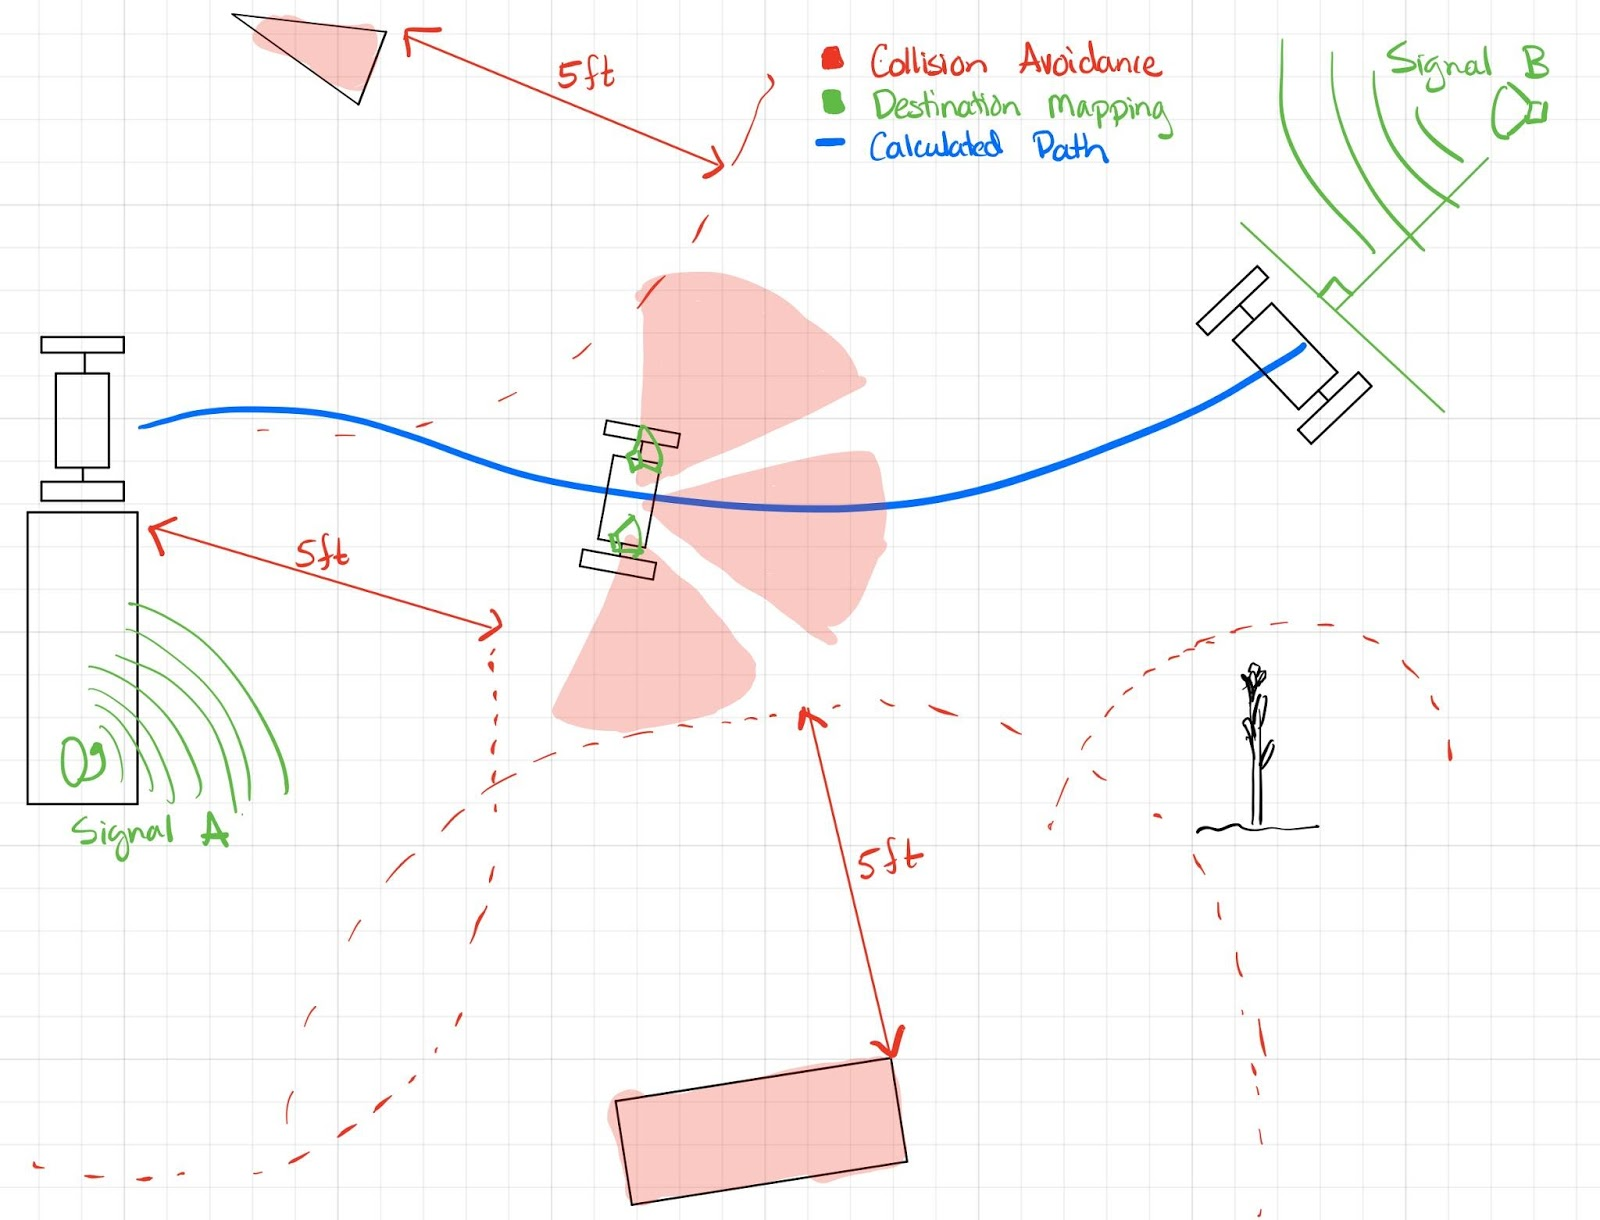
\includegraphics[width=\textwidth]{ManuverDiagram}
	\end{center}
\end{minipage}
Figure 2 helps illustrate why a sophisticated movement algorithm like SLAM would be useful for this competition. By allowing the rover to be aware of its position relative to its surroundings, it can prevent getting stuck on insurmountable obstacles and accomplish the goal of being at least five feet from the rocket with minimal driving. 

\section{Avionics}
\subsection{Design View}
The Data Logging Module involves the displaying and recording of avionics information for the rocket after sensors have recorded various streams of data during test flights.
The rocket will be equipped with, at a minimum, an altimeter for elevation measurements, a 9 degrees of freedom IMU, a barometer, and a GPS sensor. Information gathered by these sensors will be stored on a data logger called the Data Logging Module (DLM) during all test flights, and information from this data logger must be extracted and displayed in a human-readable fashion. This is separated into the following components: the in-flight data recorder operating system, the in flight data recorder software libraries, and the Graphical User Interface (GUI) to display the collected and formatted data. The in-flight recorder will interface with and record data from sensors using a BeagleBone Black microcontroller. The ground station refers to software and hardware employed to perform any post-flight data processing, and presentation that will be done on the collected data.
The DLM Ground station software must be capable of parsing and displaying the recorded in-flight data in a user-friendly and useful way. The software could be a local or remote application either viewable on the launch site or available online. Ideally, users will be able to view and explore data recorded on the launch vehicle during the flight. These statistics and figures will give the user information about how the rocket performed and raw data collected from the rocket itself. Altitude, barometric pressure, trajectory, and other pertinent information will be available for viewing by NASA adjudicators, interested students, and community members interested in rocketry. Charts and graphs will be used where applicable, data analysis will be presented with trajectory information, and raw data will be presented for sensors not requiring any analysis or sophisticated processing.
\begin{figure}[h]
	\begin{center}
		\caption{Data Logging Module data flow diagram}
		
\includegraphics[scale=0.5]{Avionics.png}
	\end{center}
\end{figure}
\subsubsection{Screen Images}
\begin{figure}[h]
	\begin{center}
		\caption{Data Logging Module website page}
		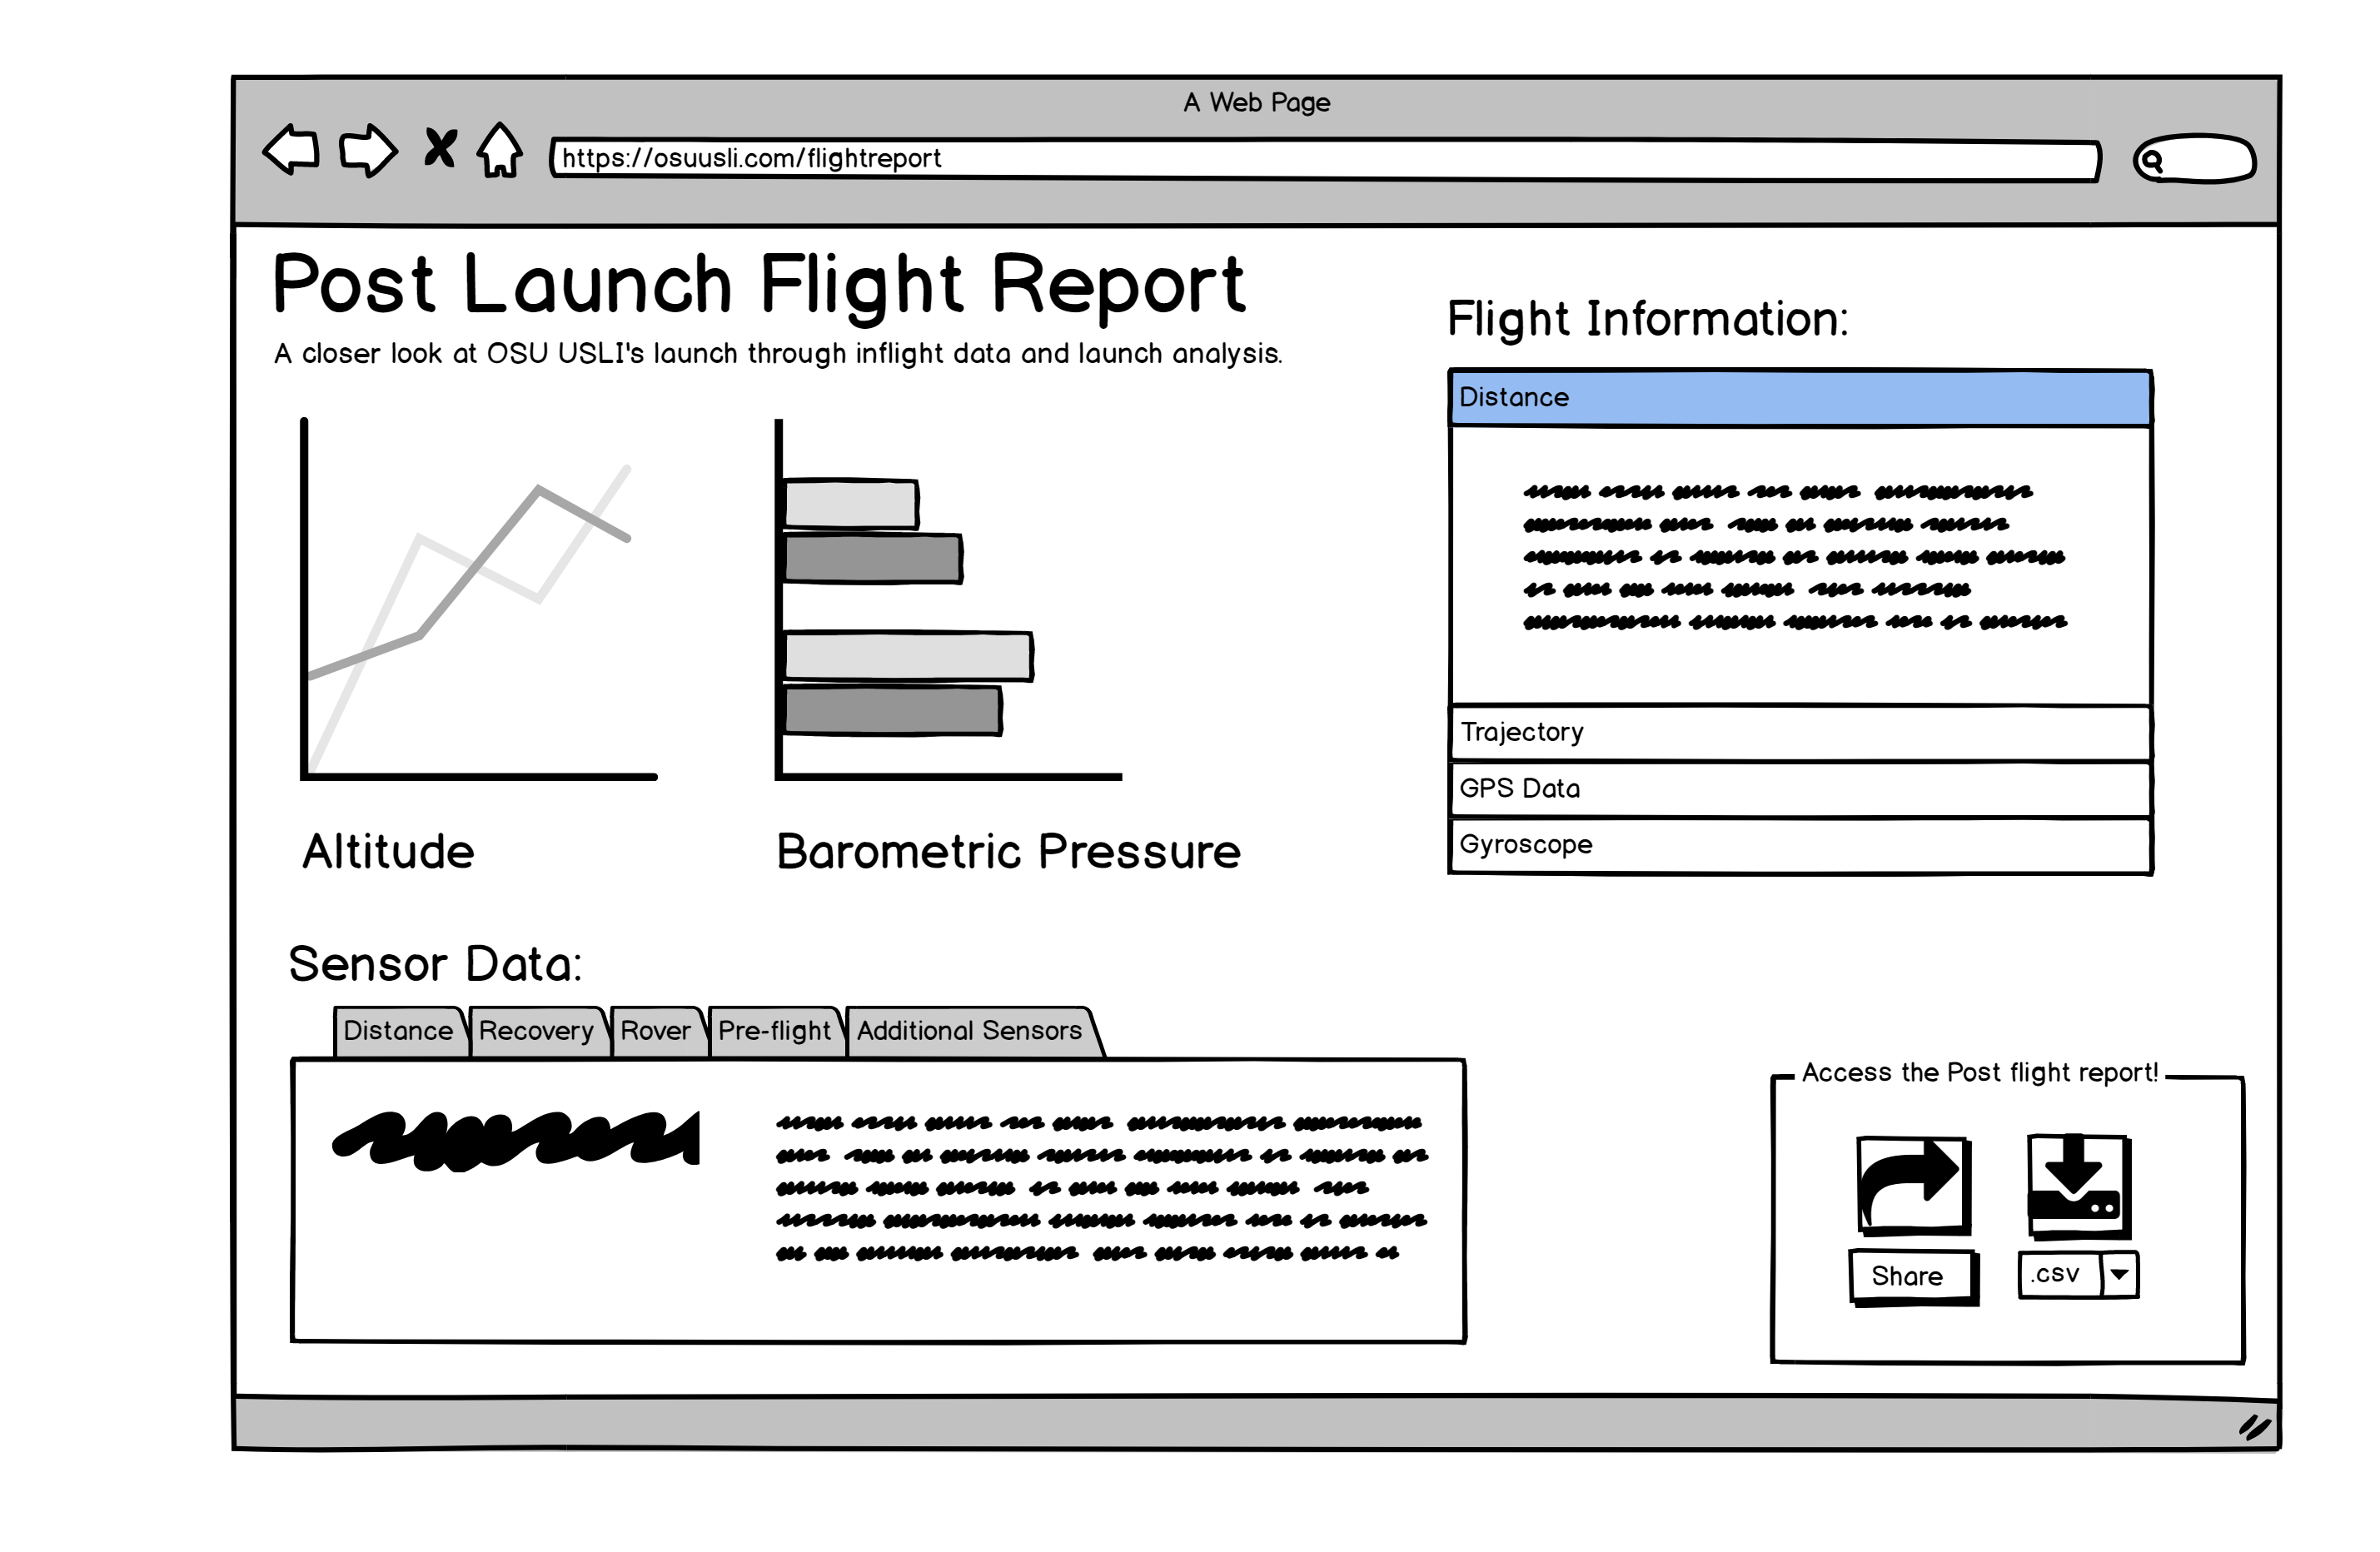
\includegraphics[width=\textwidth]{DLMGroundStationWireframe}
	\end{center}
\end{figure}
Users on the screen featured in Figure 4 will be able to expand certain menu items, like the hamburger style menu for displaying trajectory, GPS, and other data. Users will also be able to click on tabs displaying raw sensor data, with a brief description of what the sensor records in the bottom left corner. In the bottom right corner users will be able to open a modal to share a link to the page, or download/export the data as a \code{.csv} or \code{.pdf} file.

\subsection{Component design}
\subsubsection{Inertial Measurement Unit}
The IMU will use the \href{https://github.com/adafruit/Adafruit_9DOF}{AdaFruit 9 Degrees-Of-Freedom library} which will do all computations for its internal gyroscope, accelerometer, and magnetometer. This driver will send data directly and will be manipulated by the Beaglebone Black, thus recording all in-flight data.
\subsubsection{Altitude sensor}
Our current sensor for altitude (SparkFun Altitude/Pressure Sensor) is unsupported by the Adafruit libraries, so we will utilize Adafruit's \href{https://github.com/adafruit/Adafruit_Sensor}{Unified Sensor Driver}. This driver template allows us to choose a sensor type and other custom configurables for unsupported sensors and make them compatible with Adafruit I2C, USART, and other communication protocols. 
\subsubsection{Pressure sensor}
Similar to the altitude sensor, the SparkFun Pressure Sensor will also utilize Adafruit's \href{https://github.com/adafruit/Adafruit_Sensor}{Unified Sensor Driver}. The difference between the configurations will be the sensor types and sensor specific constants.
\subsubsection{Accelerometer}
The accelerometer (Adafruit ADXL377) utilizes mainly analog outputs which will need to be manually configured, calibrated, and translated to a digital output. This calibration process can be done similarly to AdaFruit's \href{https://learn.adafruit.com/adafruit-analog-accelerometer-breakouts/programming}{calibration sketch}. Then, the accelerometer data can be configured to the \href{https://github.com/adafruit/Adafruit_Sensor}{Unified Sensor Driver} to be interfaced with the AdaFruit libraries.
\subsubsection{Beaglebone Black}
The Beaglebone Black will gather information from the aforementioned sensors during the rocket flight and conduct translations to appropriate communication protocols which will then be stored in a storage device for later data processing. The logging and management of data will be done with the \href{https://github.com/adafruit/adafruit-beaglebone-io-python}{AdaFruit Beaglebone IO Python library}, which maps individual pins of the microcontroller and abstracts away some computational translations between communication protocols.

\subsection{Design Rational}
The most important aspects of an operating system for the DLM is reliability and compatibility with the BeagleBone Black. The operating system must be capable of communicating with the BeagleBone Black's GPIO and serial communication ports. A software library for the DLM must be able to make serial communication with the onboard sensors easier, while being compatible with the operating system, and the BeagleBone Black. The DLM ground station software must be capable of parsing and displaying the recorded in-flight data in a user-friendly and useful way. The data will be stored in text files, which is readable by most any language, so the GUI for the ground station is more important than the data processing itself.
\section{Website}
\subsection{Design View}
Aside from the launch vehicle and payload itself, the website serves as the main medium of giving deliverables to NASA and an excellent resource for potential USLI members to join and gain information.
\subsubsection{hosting competition documents}
All NASA specific documents will be contained in its own section of the USLI website clearly labeled as 'deliverables' containing cards to available documents. Each card will provide a link to its designated \code{.pdf} or \code{.pptx} and labeled similarly. For example each document shall be labeled in the  following order:\\\code{Oregon\_State\_University-2018-DocumentName.pdf}
\begin{figure}[h]
	\begin{center}
		\caption{Website card example}
		
\includegraphics[width=10cm]{WebsiteCardExample}
	\end{center}
\end{figure}

\subsubsection{Aesthetics}
For a clean and well designed template, the website will utilize Bootstrap's free template \href{https://startbootstrap.com/template-overviews/agency/}{agency}. This template was also chosen because of its simple styling/code as well as its vulnerability to change and customization at most web development skill levels.

\subsubsection{Team and competition specific information}
In addition to the specified 'What is it?' page, it was requested by the team leaders that a team page be provided (containing photos and emails) as well as a dynamically stretchable side bar containing links to team specific sources of information such as Trello, Google Drive, and GitHub.
\subsection{Design Rationale}
The website serves as the main medium of giving deliverables to NASA and an excellent resource for potential USLI members to join and gain information. The website itself must be simple and easy to navigate while also staying aesthetically pleasing. The website must provide the following pieces of information: competition overview, team emails photos and positions, as well as documentation and NASA deliverables.
\section{Requirements Matrix}
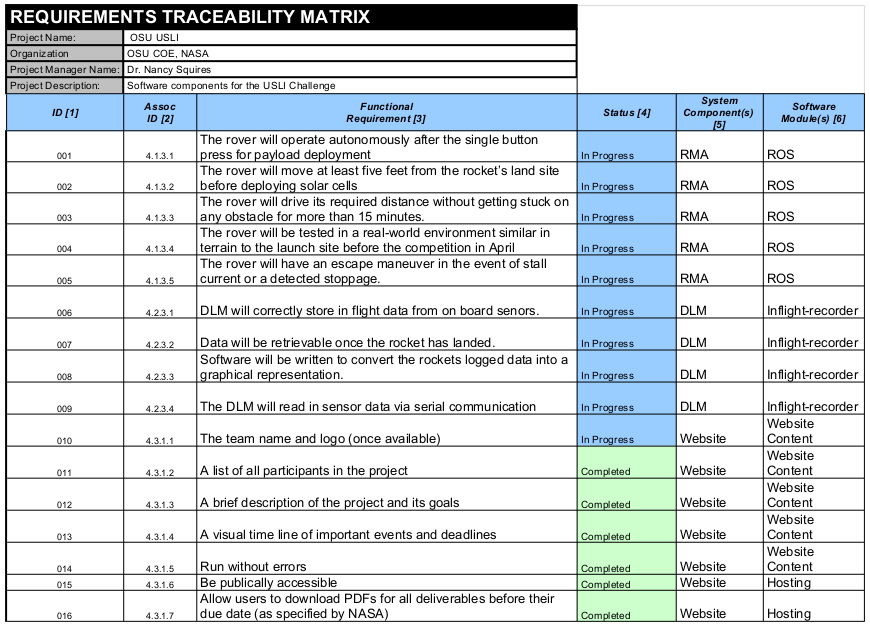
\includegraphics[width=\textwidth]{reqMatrix}
% bibliography
\nocite{*}%if nothing is referenced it will still show up in refs
\bibliographystyle{plain}
%\bibliography{bibliography}
%end bibliography

\end{document}



